\documentclass[usenames,dvipsnames]{beamer}

\usepackage{graphicx,url}
\usepackage[utf8]{inputenc}
%\batchmode
% \usepackage{pgfpages}
% \pgfpagesuselayout{4 on 1}[letterpaper,landscape,border shrink=5mm]
\usepackage{amsmath,amssymb,enumerate,epsfig,calc,xcolor,ifthen}
\usetheme{CambridgeUS}
\usecolortheme{crane}

\usepackage{empheq}


\usepackage{xcolor}
\definecolor{applegreen}{rgb}{0.55, 0.71, 0.0}
\definecolor{awesome}{rgb}{1.0, 0.13, 0.32}
\colorlet{enum1}{green}
\colorlet{enum2}{applegreen}
\colorlet{enum3}{orange}
\usepackage[most]{tcolorbox}

\tcbset{
    frame code={}
    center title,
    left=0pt,
    right=0pt,
    top=0pt,
    bottom=0pt,
    colback=blue!70,
    colframe=white,
    width=\dimexpr\textwidth\relax,
    enlarge left by=0mm,
    boxsep=5pt,
    arc=15pt,outer arc=15pt,
    }
    
\usepackage{tikz,etoolbox}
\newcommand*\mylogo{%
  \renewcommand*\do[1]{\includegraphics[height=8mm]{##1}}
  \dolistloop\mylogolist}
\newcommand*\setmylogo[1]{%
  \renewcommand*\mylogolist{}%
  \forcsvlist{\listadd\mylogolist}{#1}}
\newcommand*\addlogoleft[1]{%
  \global\let\oldmylogolist\mylogolist
  \renewcommand*\mylogolist{}%
  \forcsvlist{\listadd\mylogolist}{#1}%
  \forcsvlist{\listeadd\mylogolist}{\oldmylogolist}}
\newcommand*\addlogoright[1]{%
  \forcsvlist{\listadd\mylogolist}{#1}}
\newcommand*\mylogolist{}


\usetikzlibrary{shapes.arrows}

\def\deltaD{{D_1}}
\def\comment#1{\par\noindent\llap{$\Rightarrow$\enskip}{\bf #1}\par}
\newcommand{\bfv}{\mbox{\boldmath$v$}}
\newcommand{\bfx}{\mbox{\boldmath$x$}}
\newcommand{\bfk}{\mbox{\boldmath$k$}}
\newcommand{\bfp}{\mbox{\boldmath$p$}}
\newcommand{\bfq}{\mbox{\boldmath$q$}}
\newcommand{\bfr}{\mbox{\boldmath$r$}}
\newcommand{\bfu}{\mbox{\boldmath$u$}}
\newcommand{\bfPhi}{\mbox{\boldmath$\Phi$}}
\newcommand{\bfM}{\mbox{\boldmath$M$}}
\newcommand{\fnl}{f_{\rm NL}}
\newcommand{\gnl}{g_{\rm NL}}
\newcommand{\tdu}{\widetilde{u}}
\newcommand{\tdPhi}{\widetilde{\Phi}}
\newcommand{\tdG}{\widetilde{G}}
\newcommand{\tdP}{\widetilde{P}}
\newcommand{\tdR}{\widetilde{R}}




\definecolor{gold}{rgb}{0.95, 0.85, 0.12}

\newcommand\widecolourbox[1]{{\setlength\fboxrule{1pt}\setlength\fboxsep{8pt}\fcolorbox{red}{applegreen}{\enspace#1\enspace }}}

\newcommand\widecolourboxx[1]{{\setlength\fboxrule{1pt}\setlength\fboxsep{8pt}\fcolorbox{applegreen}{awesome}{\enspace#1\enspace }}}


\newcommand\widecolourboxxx[1]{{\setlength\fboxrule{1pt}\setlength\fboxsep{8pt}\fcolorbox{black}{orange}{\enspace#1\enspace }}}


\makeatletter
\newcommand*{\IfColorUndefined}[1]{%
  \begingroup
    \escapechar=`\\ %
    \expandafter\expandafter\expandafter
  \endgroup
  \expandafter\ifx\csname\string\color @#1\endcsname\relax
    \expandafter\@firstoftwo
  \else
    \expandafter\@secondoftwo
  \fi
}
\makeatother


\tikzset{
    myarrow/.style={
        draw,
        fill=orange,
        single arrow,
        minimum height=3.5ex,
        single arrow head extend=1ex
    }
}
\newcommand{\arrowleft}{%
\tikz [baseline=-0.5ex]{\node [myarrow,rotate=-110] {};}
}
\newcommand{\arrowright}{%
\tikz [baseline=-0.5ex]{\node [myarrow,rotate=-70] {};}
}

\newcommand{\arrowdown}{%
\tikz [baseline=-0.5ex]{\node [myarrow,rotate=-90] {};}
}
\usepackage{tikzsymbols}



\title{ {\color{awesome} Machine Learning}}
\author{\color{awesome} \bf Ben Bose}
%\institute{}
%\date{ \color{awesome} \bf  \today} 
\begin{document}


 \addtobeamertemplate{frametitle}{}{%
    \begin{tikzpicture}[remember picture,overlay]
      \node[anchor=north east,yshift=2pt] at (current page.north east) {\mylogo};
    \end{tikzpicture}}
    

\begin{frame}
 \begin{tcolorbox}
 \centering
 {\bf \Huge \color{orange} {\bf \color{awesome}  Machine Learning 1} Introduction \\ } 
 \end{tcolorbox}
 \centering
    
\includegraphics[width=8cm,height=6cm]{figs/ml_logo.jpeg}
\end{frame}

\begin{frame}
{\bf A definition: }
\centering
{\huge \emph{ ``A program learns from experience {\color{red} E} of performing task  {\color{red} T} with a performance measure  {\color{red} P}"}}  
\flushright - Tom Mitchell 1998 \\ \quad \\ \pause
The task is generally quite narrow in scope, largely because of issues in well defining a general performance measure.  --- {\color{purple} discuss}

\end{frame}


\begin{frame}{\bf Type I} 

{\bf \color{orange} Supervised learning} 
\begin{itemize}
\item
'Right' answers are known for some set of examples which we will call the {\bf training set.} This gives a well defined performance measure. \pause
\item 
Task {\color{red} T} can be a {\bf classification } problem or a continuous prediction. \pause
\item 
So many examples .... face recognition, patient diagnosis, spam detection. galaxy classification, power spectrum classification --- {\color{purple} discuss}\pause
\end{itemize}
\centering
    \includegraphics[width=10cm,height=4cm]{figs/classification.png}
\end{frame}


\begin{frame}{Type II } 

{\bf \color{orange} Un-supervised learning} 
\begin{itemize}
\item
`Right' answers are {\bf NOT} known. \emph{What is the performance measure??} \pause
\item 
Task {\color{red} T} is generally to identify trends, correlations and/or probability distributions without prior knowledge. \pause
\item 
Some examples off the top of my head  for cosmology could include identification of BAO scale from galaxy cluster data, void finding, anomaly detection? \pause
\end{itemize}
\centering
    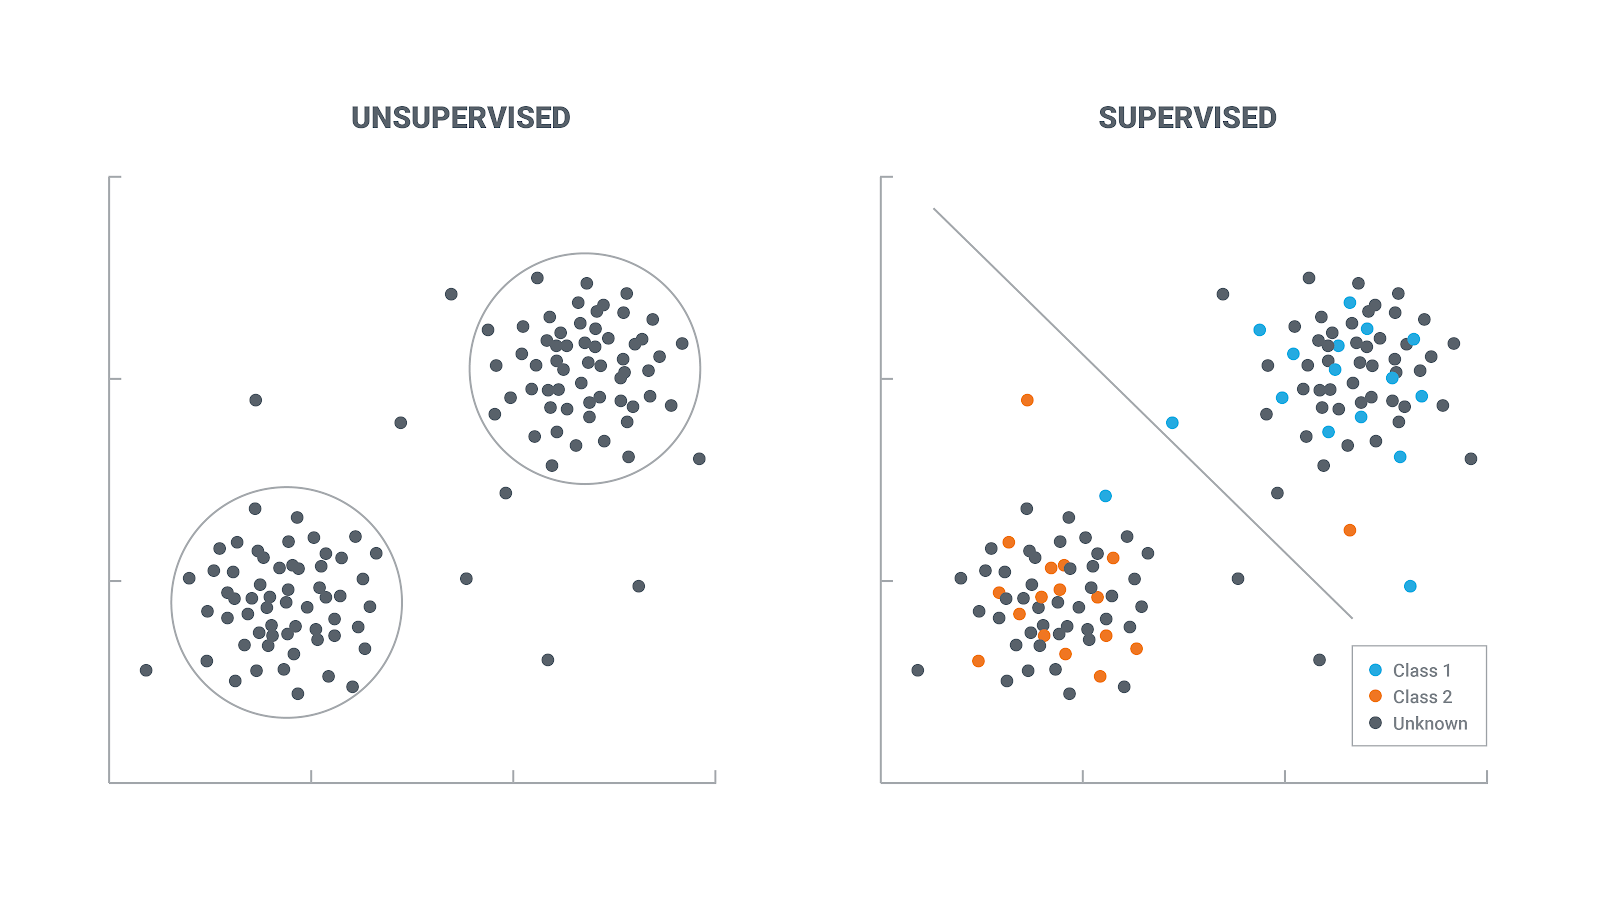
\includegraphics[width=10cm,height=4cm]{figs/unsupvssup.png}
\end{frame}


\begin{frame}{Let's focus on supervised for now} 
Let's jump right in. We will start with some definitions and notation ... \\  \pause
\begin{itemize}
\item
{\bf Features} will refer to parameters or functions of these that we choose to describe the dataset (it could be the raw data itself!).\pause
\item
{\bf Cost} will refer to the performance measure. In supervised learning, this measures how different  a prediction is from the `right' result. Denoted usually as $J$. \pause
\end{itemize}
In general I'll also use \\ 

{\bf \color{red} m: }  the number of examples we have / how large the training set is.  \\ \pause
{\bf \color{red} n: }  the number of features describing each example. \\ \pause
{\bf \color{red} $x^{(i)}$ : }  will be our feature vector for example i . \\ \pause
{\bf \color{red} $y^{(i)}$ : }  will be the correct output (class or value) for example i . \\ \pause
{\bf \color{red} theta : } will denote a vector of (fitted) coefficients that transform the feature vector into a prediction.   
\end{frame}

\begin{frame}
Let's take a super basic example... \\ 
\centering
    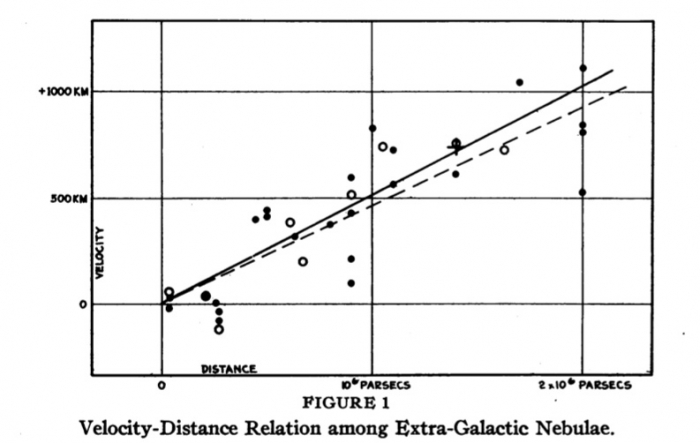
\includegraphics[width=7cm,height=4cm]{figs/class_linear.jpg} \\
Features are given by $ {\bf x} = \{1, r \}$. Say our training set is given by the points on the plot. We can just use {\bf linear regression} to get new predictions, i.e. fit a straight line. The `cost' here is just a $\chi^2$ \pause
\begin{equation}
{\rm min}_\theta  J({\bf \theta}) = {\rm min}_\theta  \frac{1}{2m} \sum_{i=1}^m \frac{({\bf \theta^Tx^i } - y^i )^2}{(\sigma^i)^2}
\end{equation}
\pause 
where in the end we would find through minimisation $\theta = \{ 0 , H_0 \}.$
\end{frame}


\begin{frame}
Just for fun and a bit of discussion, let's make a jump to {\bf polynomial /multi-variate linear} regression with a familiar example ... \\ \pause 
\centering 
    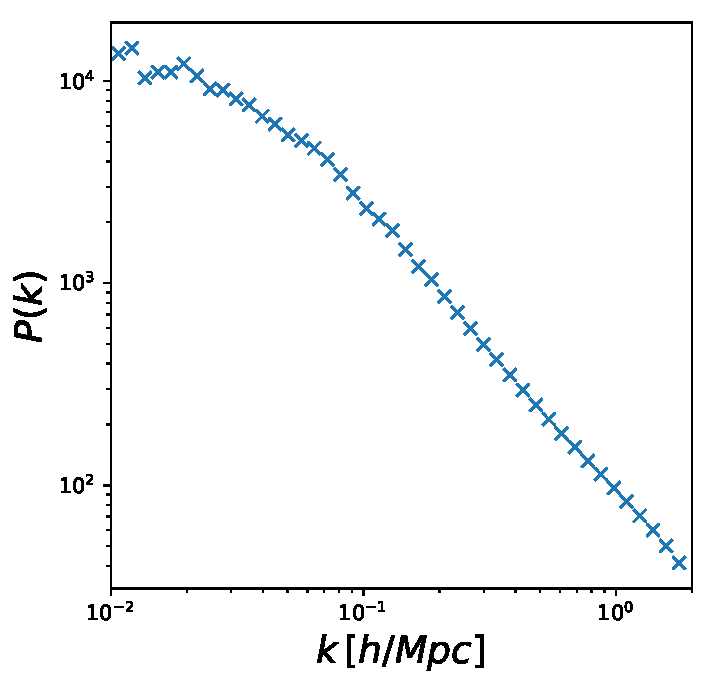
\includegraphics[width=5cm,height=4cm]{figs/pofk.pdf}
    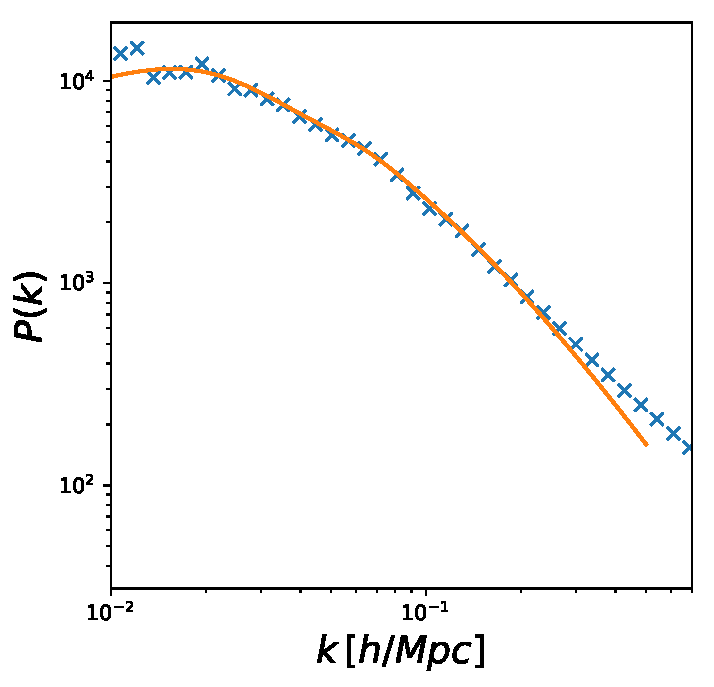
\includegraphics[width=5cm,height=4cm]{figs/pofk2.pdf} \\ \pause
In this case, {\bf \color{red} m} is the number of k-bins,  {\bf \color{red} n} is the number of features. \\
%\footnote{For $\Lambda$CDM this would be basically be $n=6 = \{\Omega_m, \Omega_b, t_0, n_s, \tau , \Delta_R^2 \}$ but would better phrased in terms of NN ?? {\color{purple} --- discuss.}}. 
Say we take ${\bf x} = \{1, k, k^2 , k^3 ...\}$
\begin{equation}
J(\theta) = \chi^2 =  \sum_{k_{\rm bins}} \frac{ [\theta^T{\bf x}- P_L^{\rm measured}(k_i)]^2}{\sigma_i^2}. 
\end{equation}
\end{frame}


\begin{frame}
{\bf A note on variance and bias using the power spectrum example : } 
\centering

  High bias:  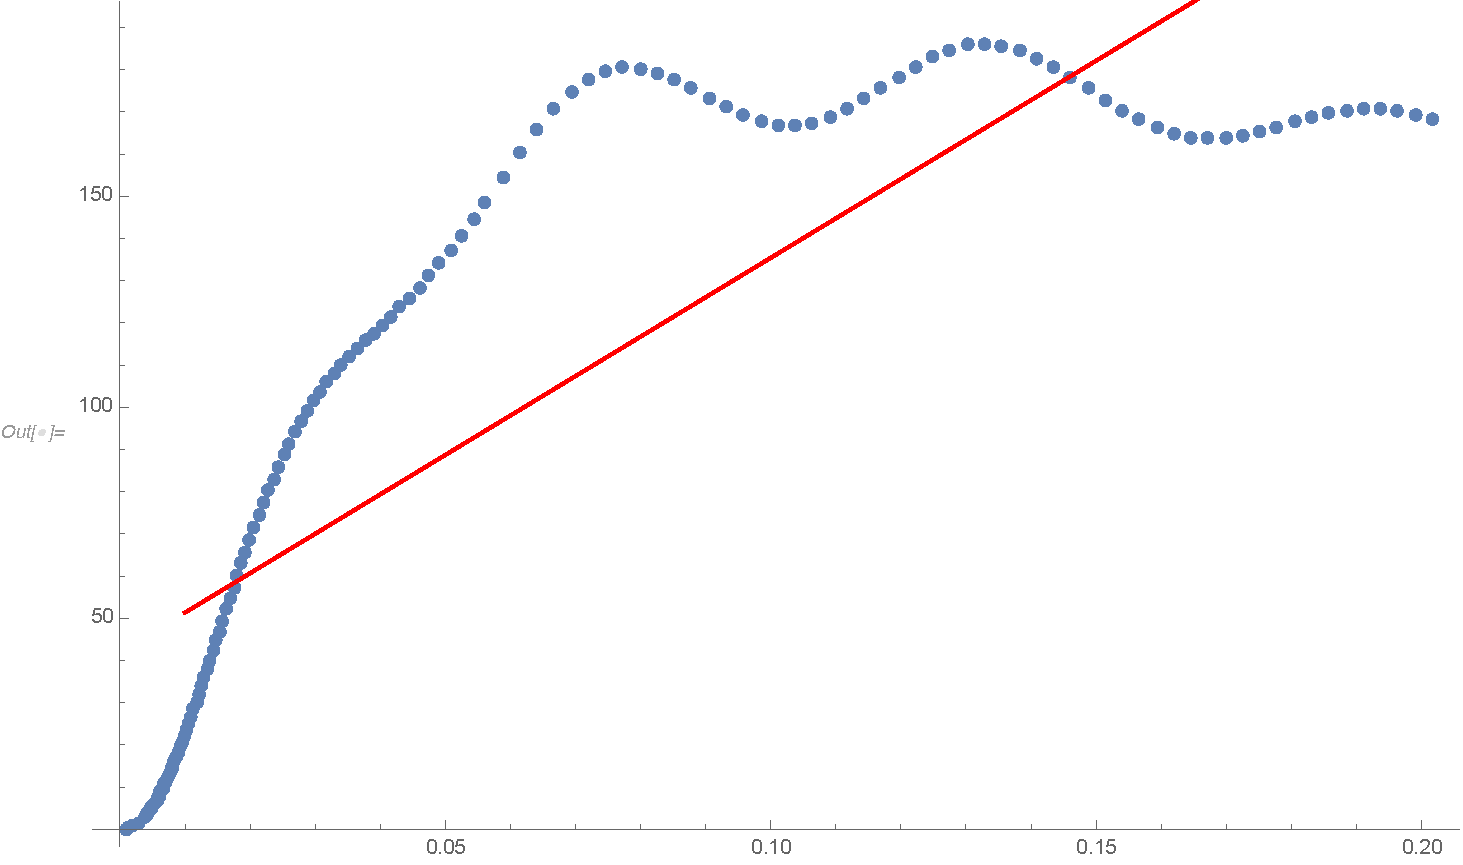
\includegraphics[width=4.cm,height=3cm]{figs/pofk_bias.pdf} \pause
    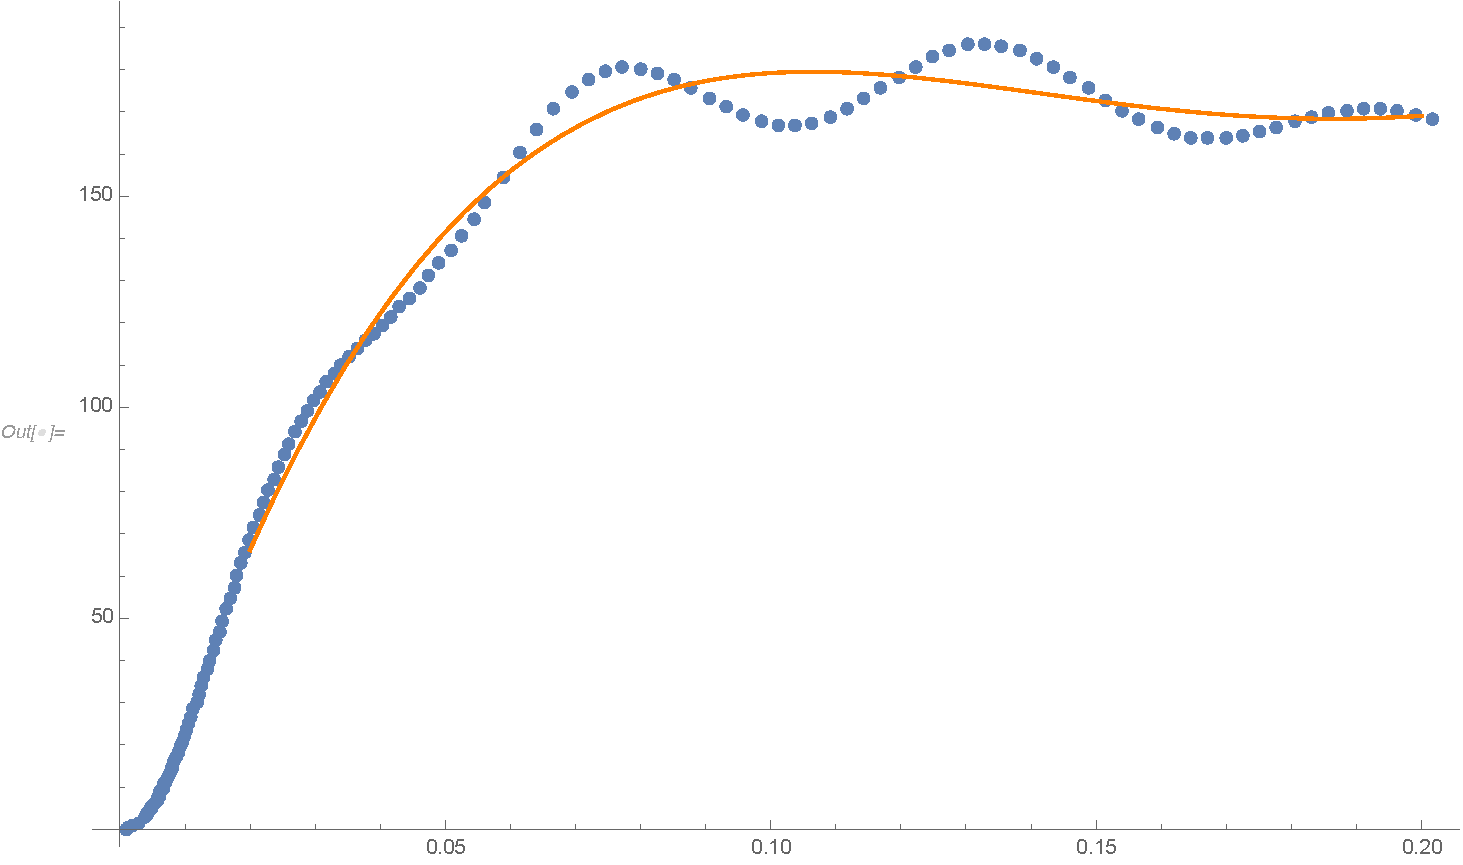
\includegraphics[width=4.cm,height=3cm]{figs/pofk_optimal.pdf} \\
         \pause
   High variance:  \includegraphics[width=4cm,height=3cm]{figs/pofk_variance.pdf}
          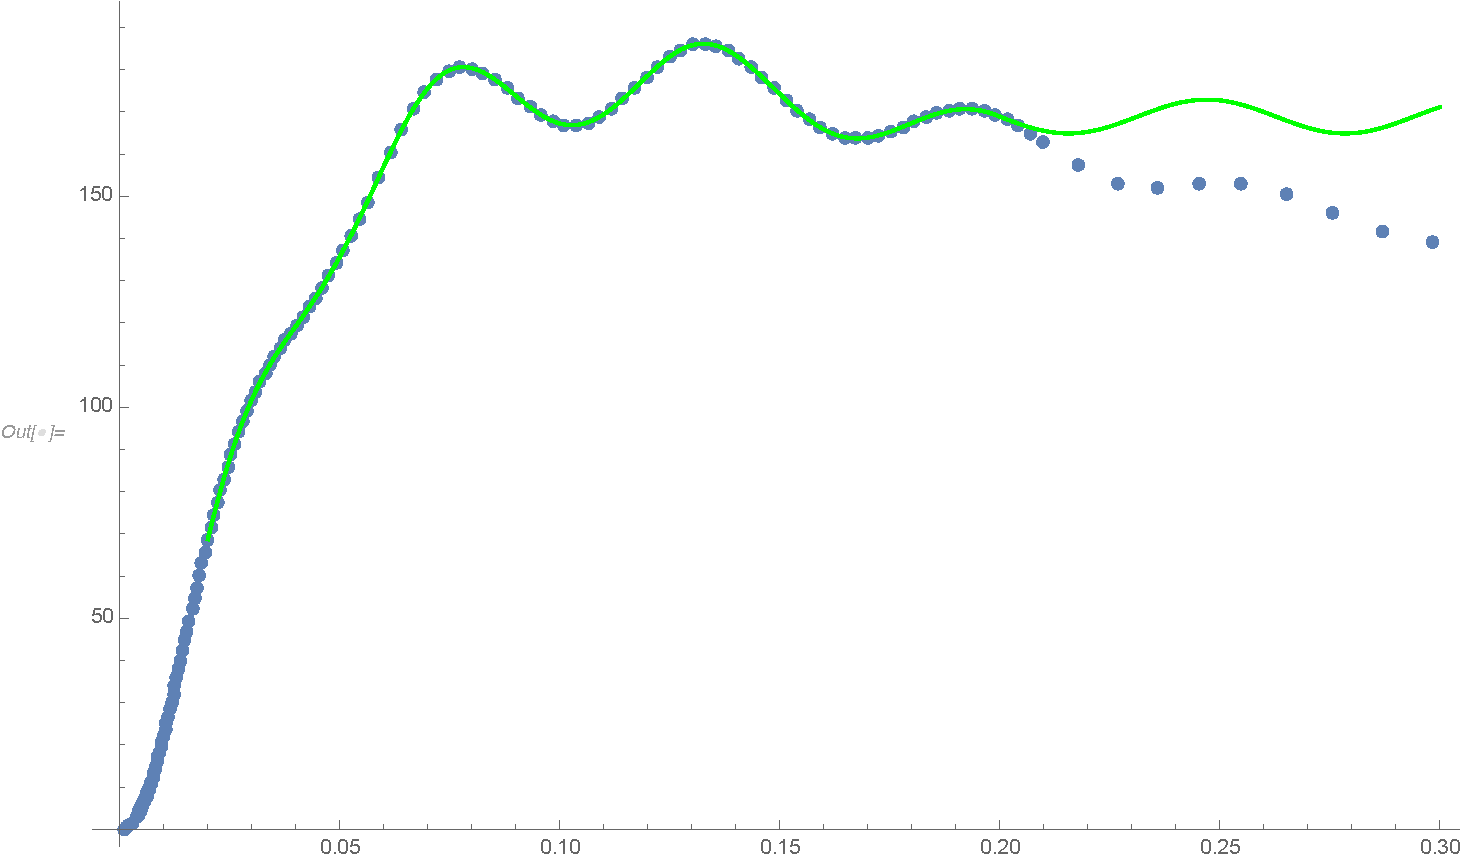
\includegraphics[width=4cm,height=3cm]{figs/pofk_variance2.pdf}


\end{frame}


\begin{frame}
Some notes before proceeding to classification problems ....  \pause
\begin{itemize} 
\item
We can minimize the cost using {\bf gradient descent} or {\bf normal equation} in practice. Many optimised packages for this in many languages. \pause
\item % Point to section IV of the review for overview of different GD methods ; remind that this is a key point in optimising NN
For polynomial regression, {\bf feature scaling} is very important - renormalise features to be of the same order  + mean normalisation ($\mu_x=0$).  \pause
%\item 
%Linear regression is terrible for classification .... obviously.
\end{itemize}

\end{frame}


\begin{frame}
What about classification? \\ 
\centering
    \includegraphics[width=10cm,height=4cm]{figs/classification.png} \\ \pause
We can use {\bf logistic regression} and the {\bf sigmoid function} to handle this. \\
    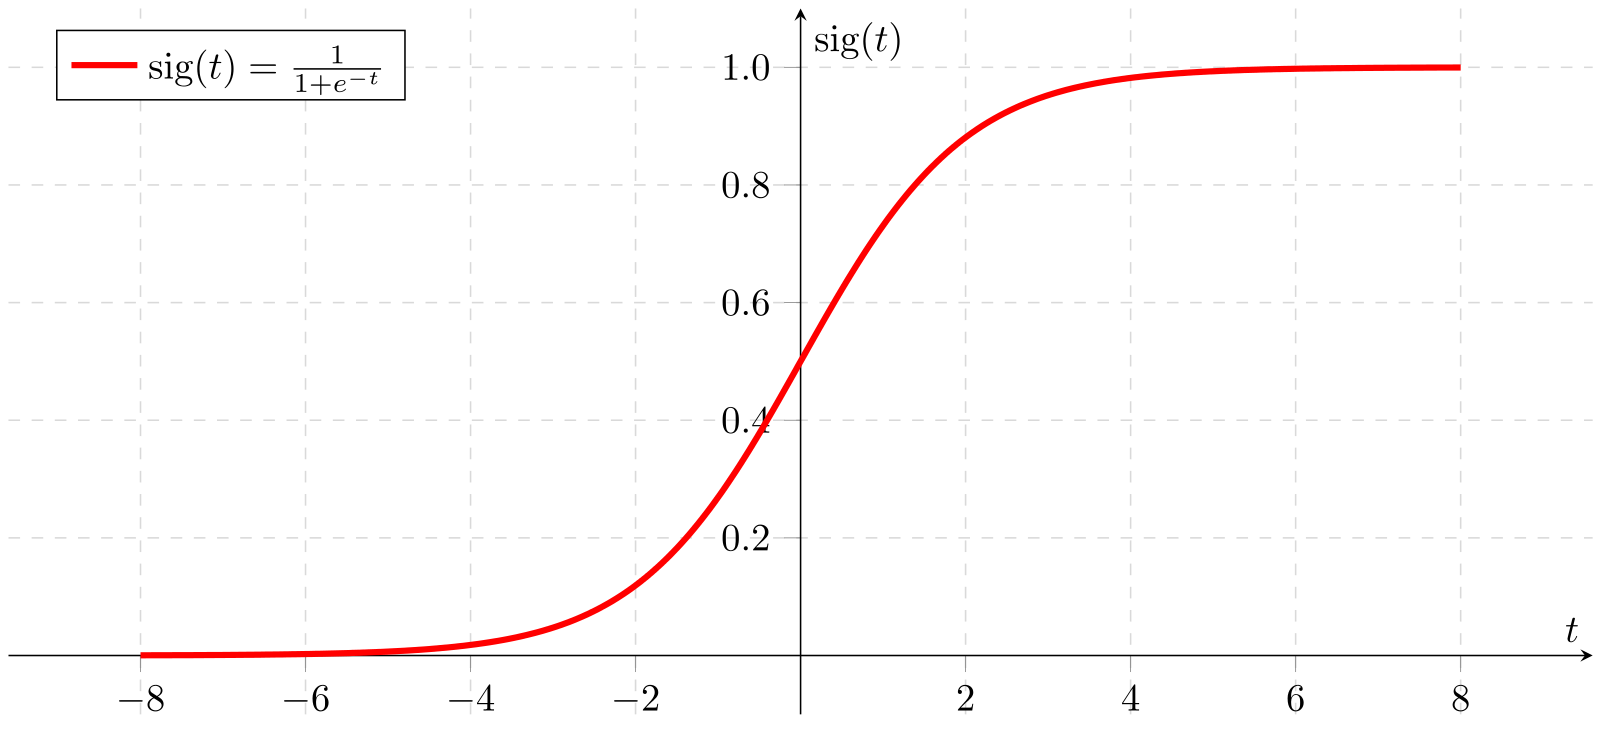
\includegraphics[width=8cm,height=3cm]{figs/sigmoid.png} \\

\end{frame}


\begin{frame}
Consider binary classification  (2 classes) 
\begin{enumerate}
\item 
Let $y=1$ (class 1) and $y=0$ (class 2)  denote the `right' answers for the two classes. 
\item
Now set our prediction to be given by  

\begin{columns}
\column{5cm}
 \[   
h({\bf \theta^T x}) = 
     \begin{cases}
       1 &\quad\text{if $sig({\bf \theta^T x})$ } \ge 0.5 \\
       0 &\quad\text{if $sig({\bf \theta^T x})$ }  < 0.5 \\
     \end{cases} \quad ,
\]

\column{5cm} 
 \[   
y = 
     \begin{cases}
       1 &\quad\text{if ${\bf \theta^T x}$ } \ge 0.5 \\
       0 &\quad\text{if ${\bf \theta^T x}$ }  < 0.5 \\
     \end{cases}
\]
\end{columns}
\pause
${\bf \theta^T x}$ then draws out what is called the {\bf decision boundary}. 
\centering
    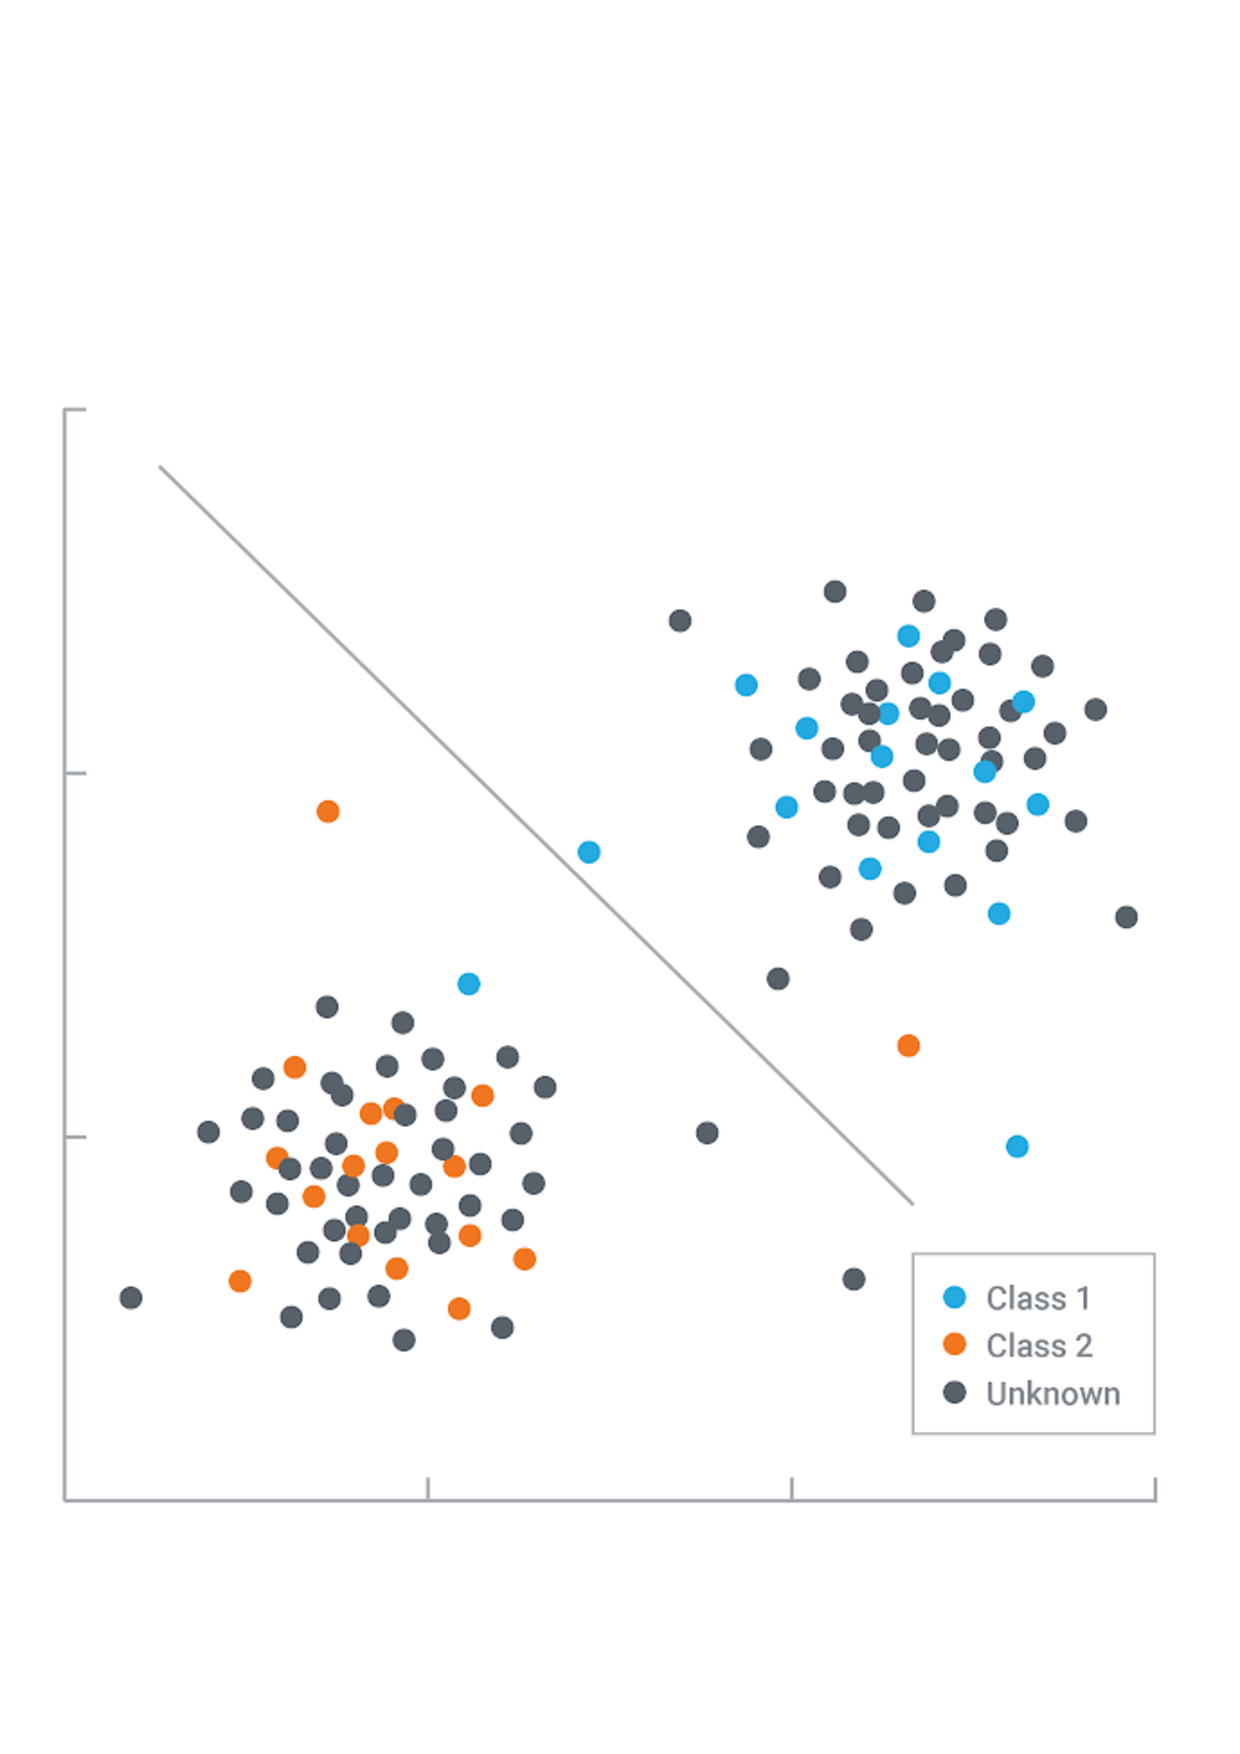
\includegraphics[width=4cm,height=4cm]{figs/supervised.pdf} \\

\end{enumerate}
\end{frame}



\begin{frame}
Some notes to  bring this all together 
\begin{itemize}
\item
Can use {\bf polynomial features} to get complicated decision boundaries.  \pause 
\item
Should not use least square error for the cost because sigmoid is non-linear and makes the cost {\bf non-convex} --- hard to find global min.\footnote{see Week 3, Cost Function of Cousera}
\begin{equation}
J(\theta) = \frac{1}{m} \sum_{i=1}^m \left[ y^i \log[h({\bf \theta^T x^i})] + (1-y^i)\log[1-h({\bf \theta^T x^i})] \right]. \pause
\end{equation}
\item
For multi-class classification, we can use the {\bf one vs all} method: 
\begin{enumerate}
\item
Delimit classes numerically as $\{0,1,2,3, .... k\}$.
\item
Train for k-sets of optimised $\theta$, one for each class.
\item
 For a new example $\bar{\bf x}$, choose the class $j$ that gives the maximum value of $sig({\bf \theta^T_j \bar{\bf x}})$.
 \end{enumerate}
\end{itemize}
\end{frame}

\begin{frame}{Example 1: Spam classifier} 
\centering
    
\includegraphics[width=4cm,height=4cm]{figs/spam.jpeg} \\  \pause
Features could be word frequency or appearance:  $x_j = 1,0$ if some word appears or not. \\
Then $\theta^T x^i = \theta_0 + \theta_1 x_1^i + \theta_4 x_4^i .... $ etc. \\ \pause
If we want to include frequency, then we might set $x_j = n_j$ where $n_j$ is the number of times the $j^{th}$ word appears. 

\end{frame}

\begin{frame}
{\huge  \bf Summary so far: } 
\begin{itemize}
\item
Machine learning can be classified as supervised and unsupervised learning. \pause
\item 
In supervised learning we have the answers in the form of a training set. The correct answer could be a predicted value or a classification. \pause
\item
We can form a hypothesis for the prediction or classification using linear/polynomial regression OR logistic regression + one vs all. \pause
\item
Feature selection is very important!
\end{itemize}
\end{frame}

\begin{frame}{Example 2: Puzzle classifier } 
\centering
    \includegraphics[width=5cm,height=4cm]{figs/classification.jpg} \pause
        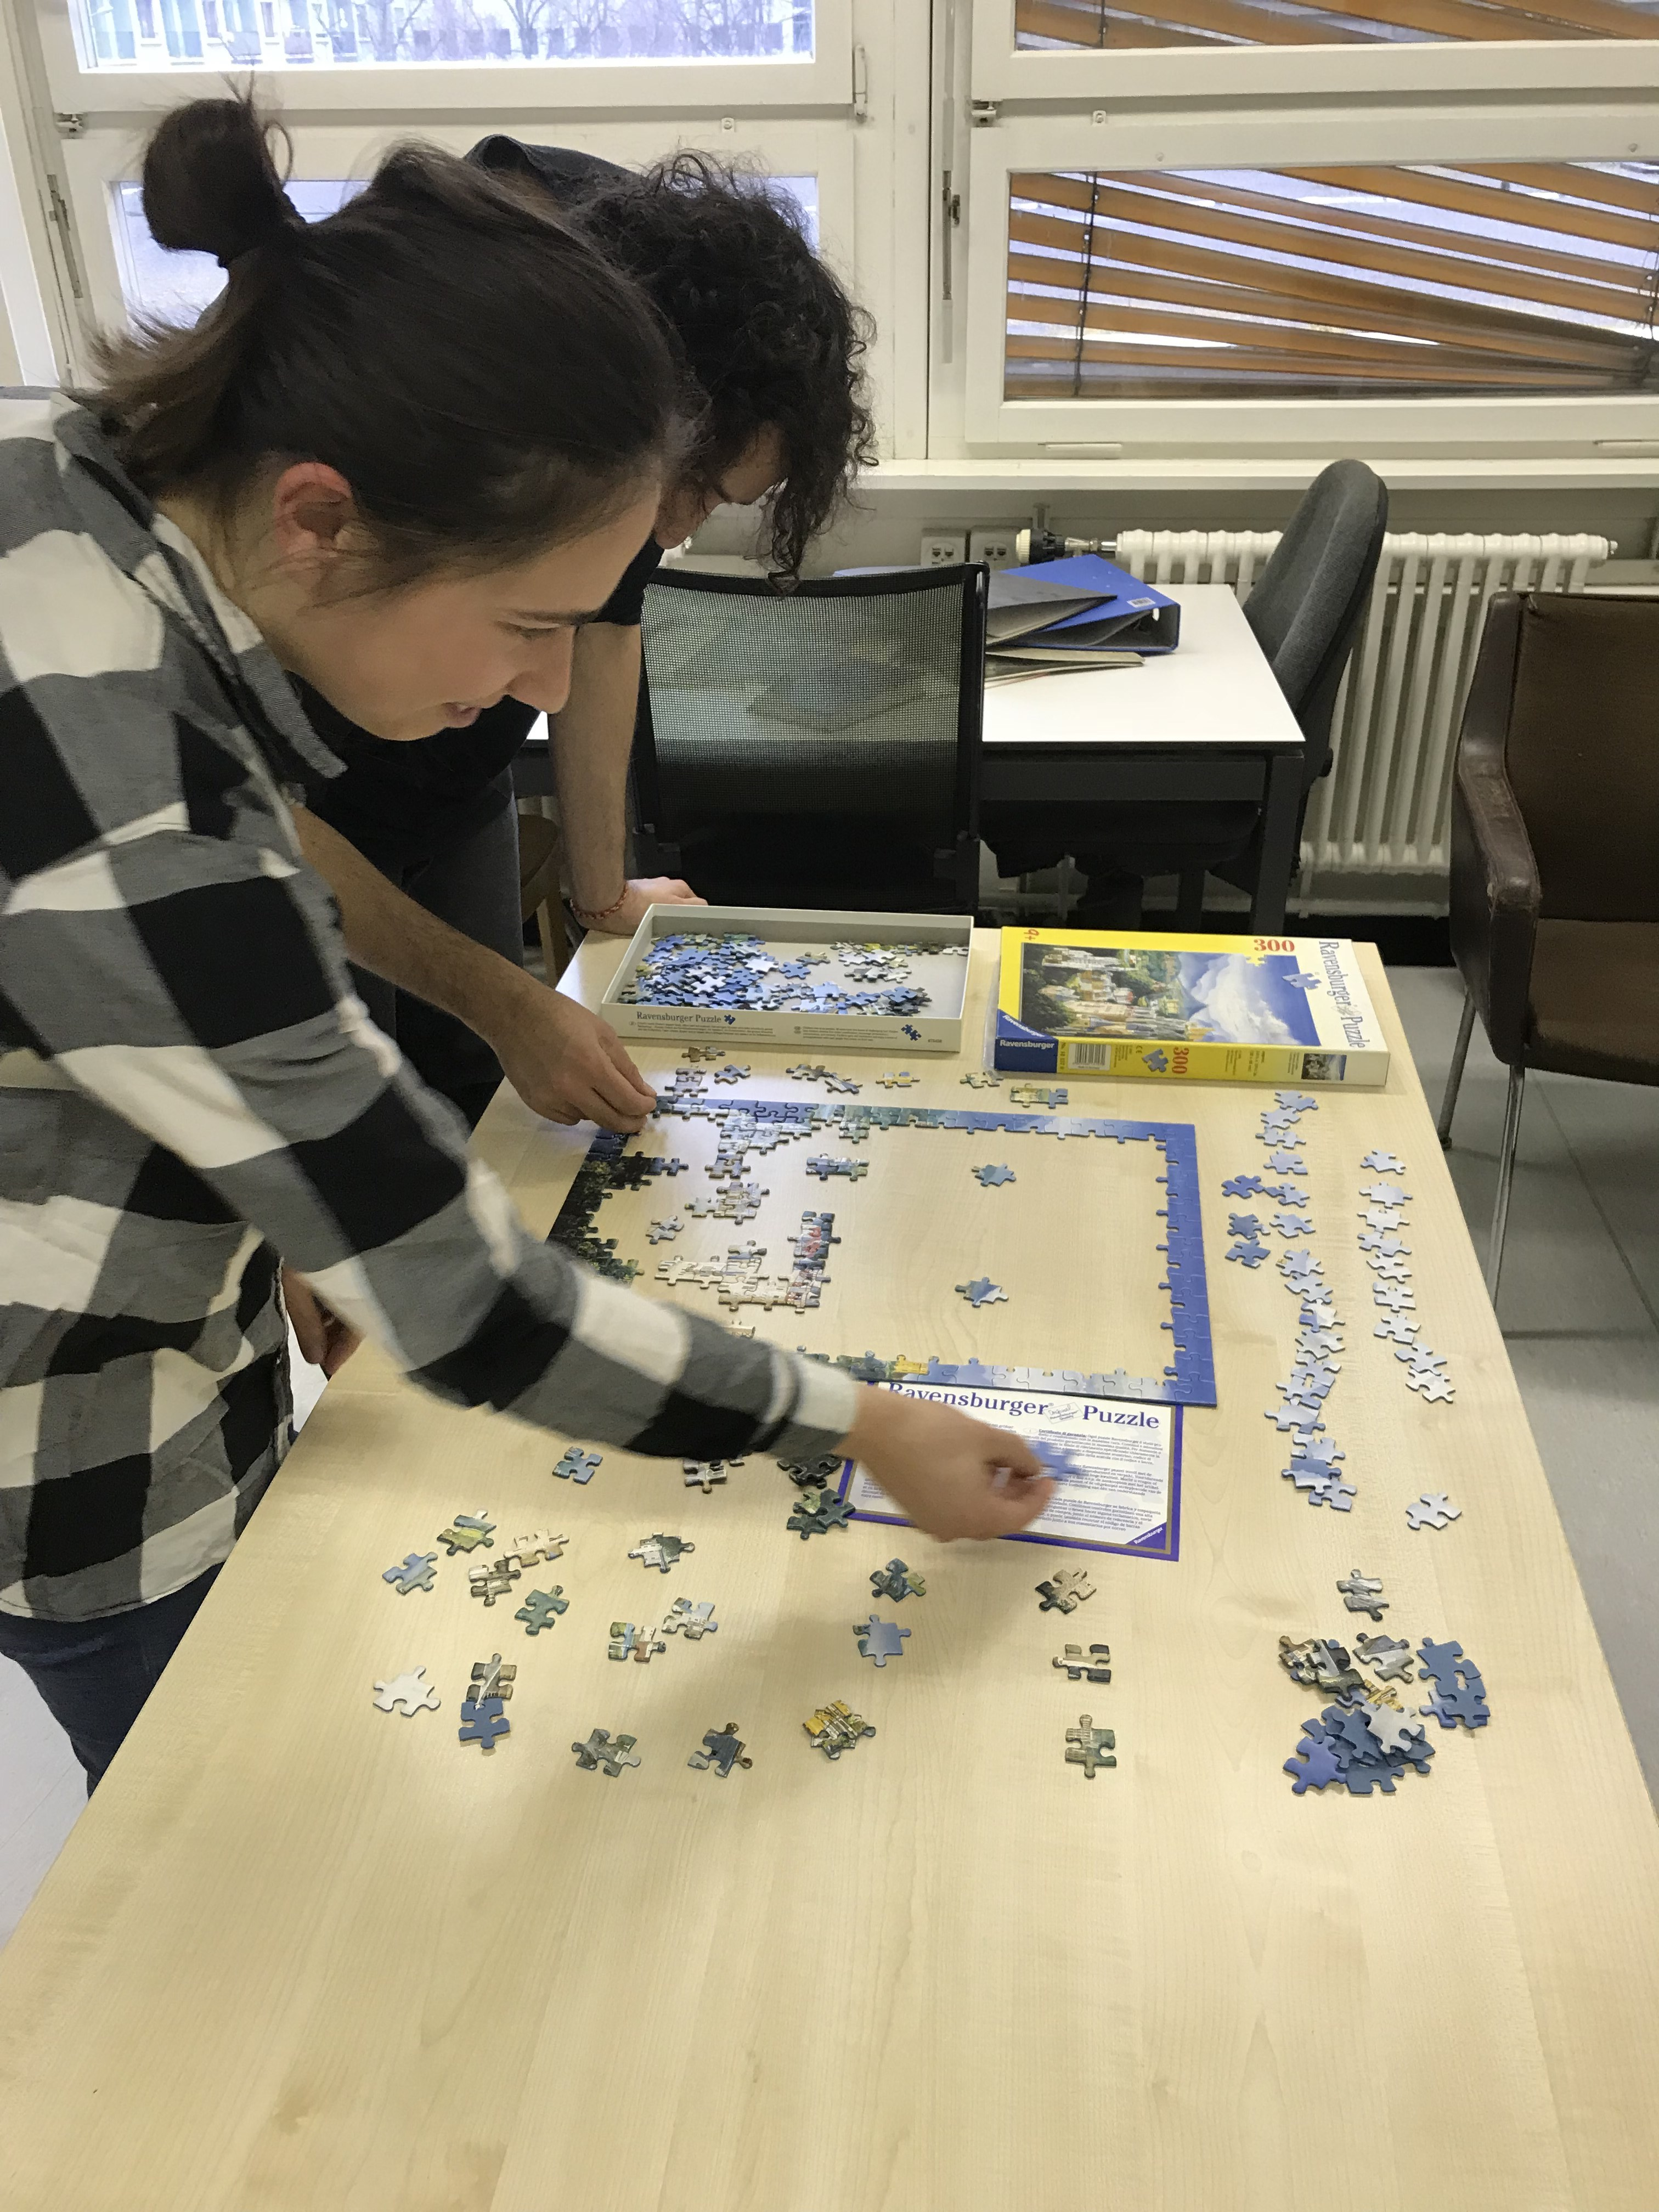
\includegraphics[width=5cm,height=4cm]{figs/ml_coffee.jpg} \\  \pause
   Features are shades of blue: 
 \begin{itemize}
 \item
  $x_j = 1,0$ if average of pixels on a piece are in some blue category j.  
  \item
  $x_j = \bar{B}$ in RGB context. We should rescale/normalise this feature.  
\end{itemize}

\end{frame}

\end{document}



